\chapter{Application of Neural Networks for Object Detection}
In recent years, the evolution of hardware allowed for the creation of deep neural networks (DNNs) for multiple purposes. Eventually, image processing has become one of the fields where DNNs outperformed traditional and machine learning approaches. 

\todo{bla}
NNs vs ML
Define (NNs) abbr.
softmax
perform object detection via bounding box localization
augmentation - data size

\section{Metrics}
In order to evaluate and compare multiple approaches, we require clearly defined metrics. A state-of-the-art model presented without full specification of used evaluation metrics makes comparing multiple such results impossible. Thankfully, there are clearly defined competitions and challenges with precisely defined rules that are often used to make such comparisons. 

The \textit{ImageNet Large Scale Visual Recognition Challenge (ILSVRC)}\footnote{\url{http://www.image-net.org/challenges/LSVRC/}} is most often used to benchmark classification. Object detection is commonly evaluated in two challenges: the \textit{PASCAL Visual Object Classes Challenge}\footnote{\url{http://host.robots.ox.ac.uk/pascal/VOC/}}, and the \textit{COCO Object Detection Task}\footnote{\url{cocodataset.org/}}. Each challenge also provides a public dataset, \textit{ImageNet}, \textit{VOC}, and \textit{COCO} respectively.

In this section, we define metrics used to evaluate those challenges, but also other, not considered qualities. Most notably, none of the challenges mentioned is evaluated based on the speed of the model. Because our work focuses on real-time video analysis, we are interested in finding a balance between accuracy and the number of images processed per second (fps). One more factor to consider would be the physical size of the model, usually represented by the number of parameters and directly impacting the amount of needed memory.

\subsection*{Classification}
The most common and intuitive evaluation metric for classification problems is the number of correctly classified samples as a ratio of all samples. This ratio is referred to as a \textbf{classification accuracy}. However, a complement to the accuracy, \textbf{top-1 error}, is also often used. In \textit{ILSVRC},  alongside top-1 error, a \textbf{top-5 error} is used as another criterion. The top-5 error represents the fraction of test samples in which the correct label does not appear in the top 5 predicted results.

\subsection*{Object detection}
Multiple objects in each image, make object detection more complex task than classification. First of all, there is no simple one-to-one mapping between ground-truths and detections, like in the case of classification. A ground-truth data are a set of \textit{N} boxes with labels, and predictions generate a set of \textit{M} boxes with labels and confidence values. At this point, predictions can be filtered by a confidence threshold and non-maximum suppression (NMS). NMS is a post-processing algorithm responsible for merging all predictions that belong to the same object. 

Because predicted boxes do not perfectly match ground-truths, a matching algorithm is needed to decide whether a prediction is true positive or false positive. Matching is determined by computing intersection over union (IoU) value for each pair of ground truth and predicted boxes. Predictions with IoU lower than predetermind threshold are ignored.
$$\text{IoU} = \frac{\text{Area}(\text{Prediction} \cap \text{Ground truth})}{\text{Area}(\text{Prediction} \cup \text{Ground truth})}$$

With predictions sorted into true positives (TP), false positives (FP) and false negatives (FN) (no predictions matching a ground-truth box) we are able to calculate \textbf{precision} and \textbf{recall}.
$$\text{Precision} = \frac{\text{TP}}{\text{TP}+\text{FP}} = \frac{\text{TP}}{\text{All predictions}}$$
$$\text{Recall} = \frac{\text{TP}}{\text{TP}+\text{FN}} = \frac{\text{TP}}{\text{All ground truths}}$$

With precision and recall defined, we can define the first metrics used for object detection. Note that all following metrics depend on IoU threshold.

\subsubsection{Precision-Recall curve}
Precision-Recall curve (PR curve) is a curve plotted for a specific class and shows the changes in precision and recall as the confidence level changes. Points on the PR curve are determined by sorting the predictions by the confidence score and for each prediction also considering all objects above its confidence score, then calculating the resulting precision and recall for those predictions. An object detector of a particular class is considered reliable if its precision stays high as recall increases, meaning precision is good with lower confidence threshold.

\subsubsection{Average Precision (AP)}
Comparing curves is not an easy task, particularly if they cross each other frequently, as it often happens with PR curves. AP is a numerical metrics representing area under the PR curve. It is calculated by interpolation, either on all data points or on 11 equally spaced points.

Interpolation equation for all points:
$$\sum_{r=0}^1 (r_{n+1} - r_n ) p_{interp}(r_{n+1})$$
with
$$p_{interp}(r) = \max_{\Tilde{r} \geq r} p(\Tilde{r})$$
where $p(\Tilde{r})$ is precision at recall $\Tilde{r}$.

\subsubsection{Mean Average Precision (mAP)}
Finally, the mAP is the number we can most often see as the performance metrics of object detectors. As the name suggests, it is a mean of AP across the classes. Most common notation mAP@[0.5] means mAP with IoU threshold 0.5. The mAP can also be averaged over multiple IoU thresholds, mAP@[.5, .95] represents the average mAP from IoU 0.5 to 0.95 usually with step 0.05.

\subsection*{Inference time}
Inference time is usually a small number in milliseconds that is not directly applicable to our problem. Our task is to process a large number of images. Therefore a number of processed \textbf{frames per second} (fps) is more natural metrics. Value of fps is always averaged. However, unlike precision metrics, the fps values are heavily dependant on hardware, batch size and amount of pre- and post-processing included in the measurement. Therefore, only the measurements done in the identical hardware and software environment can be directly compared.

\section{Classification networks}
\label{sec:clsnets}
To better understand detection networks, we shortly describe their predecessors, classification networks. Classification network is a convolutional neural network (CNN) \cite[ch.~9]{bib:dlbook} that given an image, returns a confidence score of correspondence to each of the classes. Usually, soft-max function is applied to the confidence score to represent a probability distribution. A commonly used benchmark for the accuracy of such networks is the \textit{ILSVRC} challenge.
The \textit{ILSVRC} challenge is usually used to benchmark the accuracy of such networks.

In \cref{sec:detnets}, we show how classification models are used as a backbone for a detector network.

\subsection{AlexNet (2012)}
A significant breakthrough in use of CNNs happened in 2012, when the \textit{AlexNet} \cite{bib:alexnet} won the \textit{ImageNet} image recognition challenge. It was the first time a deep CNN performed better than traditional computer vision and machine learning approaches. 

\textit{AlexNet} has a simple architecture with five convolutional layers and two fully connected layers, followed by a softmax layer. It has created a foundation on which today's state-of-the-art models are built and set a new standard for image recognition.

\subsection{VGG (2014)}
\label{sec:VGG}
The network architecture, mostly known as \textit{VGG} \cite{bib:vgg}, pushed the concept of AlexNet even further and has proved the feasibility of deep network with small convolutions. 

Each of the \textit{VGG's} convolutional filters uses 3$\times$3 kernel, and the depth of the filters is increased through the network, reaching 512 filters in the last layers. Three fully connected layers and softmax are applied after the convolutions, see \cref{tab:vggarch}. There are multiple versions of the \textit{VGG} architecture, depending on the number of convolutional layers, the most popular is the 16 layer version. 

\textit{VGG} network is considered a general architecture for a classification network due to its linear architecture with decreasing size of the features and increasing number of channels. 

\begin{table}
    \centering
    \rotatebox{90}{
        \vggArch
    }
    \caption{Architecture of VGG network, version D. Taken from \cite[table 1]{bib:vgg}}
    \label{tab:vggarch}
\end{table}
    
\subsection{Inception (2014)}
\label{sec:inception}
Previous architectures showed that increasing the number of layers and layer size, leads to better precision. \textit{Inception v1} \cite{bib:googlenet}, also known as \textit{GoogLeNet}, aims at increasing precision while improving utilization of computing resources.

A growing cost of stacking more convolutional layers can quickly overpower the benefits of increased accuracy. This network introduces the concept of sparsity by using the \textit{inception modules} \cref{fig:incept_mod}, to avoid the aforementioned cost. A sparse structure is approximated by using multiple convolutions with different kernel sizes and concatenating the outputs together. Max-pooling is also performed as an alternative to convolutions and concatenated to the output. Because high dimensional convolutions are costly, a reduction to the channels is introduced by using 1$\times$1 convolution as a preceding layer.

The network is then formed by linearly stacking nine inception modules, preceded by a linear stem network and followed by a fully connected classifier. Two auxiliary classifiers are added to intermediate layers of the network to help propagate gradients and provide regularisation during the training.

A set of improvements to the \textit{Inception} network was introduced in later versions of the network. Most notably a factorization of convolution layers was introduced in Inception v2 and v3 \cite{bib:inception2}.


\begin{figure}
    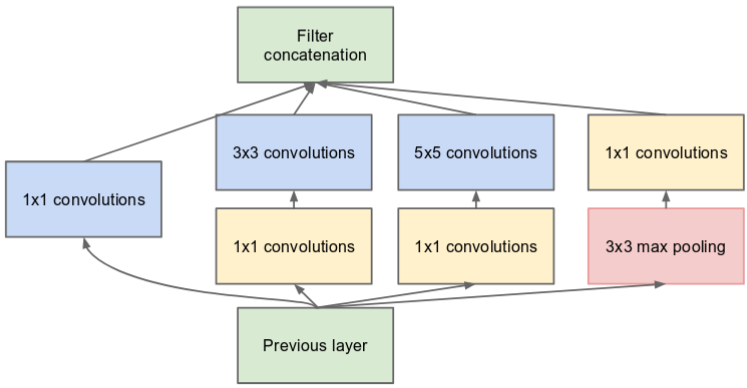
\includegraphics[width=\textwidth]{img/inception}
    \caption{Inception module, picture from \cite[figure 2]{bib:googlenet}.}
    \label{fig:incept_mod}
\end{figure}

\subsection{ResNet (2015)}
\label{sec:resnet}

Although it has become possible to train deeper and deeper CNNs, degradation has eventually been observed. Adding more layers to models started to produce higher training error. Theoretically, adding more layers to a smaller model should produce at least equal results, as the smaller model is the subspace of the larger one. A solution to this problem was proposed in the ResNet architecture, by directly introducing identity functions to the network \cite{bib:resnet}.  

A baseline of \textit{ResNet} is directly inspired by \textit{VGG} (\cref{sec:VGG}). Most of the convolutional layers have 3$\times$3 filters and follow two simple rules: keep the number of filters the same, unless changing the output size and double the filters if the feature size if halved. A residual connection is then added to each pair of the convolutional layers. This connection is either an identity or a projection done by 1$\times$1 convolution to match the increased number of filters. 

\begin{figure}
    \resnetArch
    \caption{Architecture of the ResNet network and residual blocks. Each of the four \textit{Layers} are created by stacking multiple residual blocks.}
    \label{fig:resnet_arch}
\end{figure}

We can see the high level architecture of this model in \cref{fig:resnet_arch} (left). Each of four \textit{Layers} is composed of multiple linearly stacked residual blocks, exact numbers of blocks can be found in \cite[table 1]{bib:resnet}. A feature map size is preserved inside each of the \textit{Layers} and halved between them. A type of residual block we described previously was a \textit{Basic block} with two convolutional layers and is used for smaller \textit{ResNet} models (ResNet-18, ResNet-34). Deeper \textit{ResNet} models (ResNet-50, ResNet-101, ResNet-152) use the \textit{Bottleneck block} with three convolutional layers, where the 1$\times$1 layers are responsible for reducing and then restoring dimensions, leaving the 3$\times$3 layer a with smaller input and output dimensions. Remarkably, the 152-layer \textit{ResNet} has lower complexity than the 16-layer \textit{VGG} network.



\subsection{Xception (2017)}
\label{sec:xception}
Xception architecture \cite{bib:xception} is heavily inspired by previous architectures, mainly \textit{Inception} and \textit{ResNet}. It is built on the hypothesis that "the mapping of cross-channel correlations and spatial correlations in the feature maps of convolutional neural networks can be entirely decoupled." This hypothesis expands upon the hypothesis underlying \textit{Inception} architecture. Therefore the name \textit{Extreme Inception}. 

The hypothesis is realized in the form of depthwise separable convolution layers. Depthwise separable convolution consists of two steps: a depthwise convolution and pointwise convolution. A depthwise convolution is a convolution performed independently over each channel, i.e., a convolution without changing the number of channels. The second step is a pointwise convolution that uses 1$\times$1 kernel to map the input channels into new channel space.

The architecture is created by linearly stacking convolutional layers with the addition of residual connections as seen on \cref{fig:xception}. Convolutional layers, non-linearity, and poolings are structured into residual blocks similarly to \textit{ResNet} architecture.

\begin{figure}
    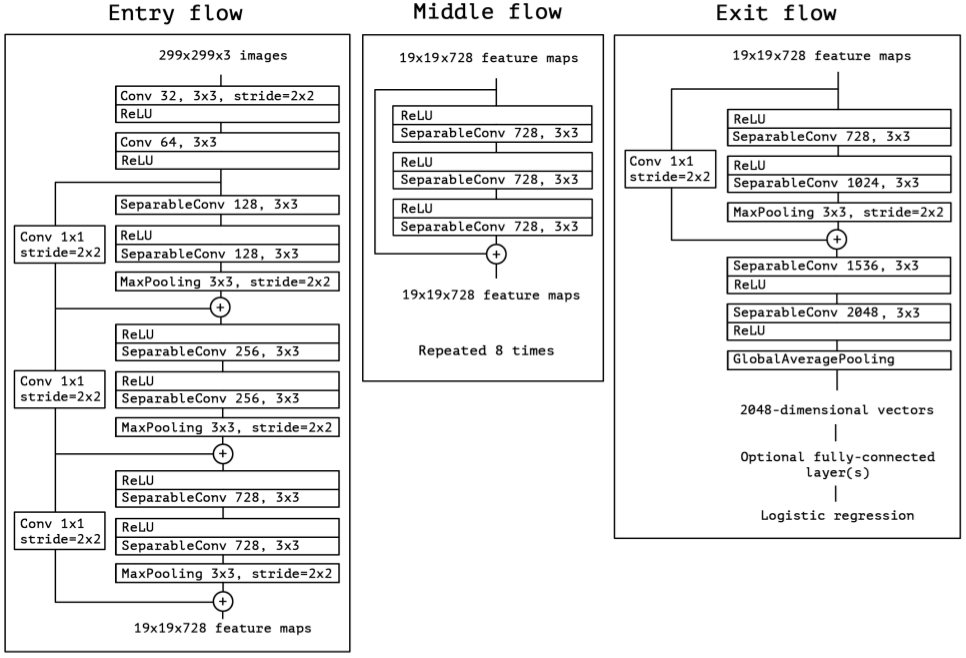
\includegraphics[width=\textwidth]{img/xception}
    \caption{Structure of \textit{Xception} architecture. Taken from \cite[fig. 5]{bib:xception}.}
    \label{fig:xception}
\end{figure}


\subsection{NASNet (2017)}
\label{sec:nasnet}
The difference between this architecture and the others mentioned is that \textit{NASNet} \cite{bib:nasnet} was designed by a machine learning algorithm. It is a result of a \textit{AutoML}\footnote{https://ai.googleblog.com/2017/05/using-machine-learning-to-explore.html} project that automates the design of network architecture. Unlike manually designing the network by trial and error, \textit{AutoML} searches space of all possible models, e.g., using reinforcement learning and evolutionary algorithms. The downside of this approach is the computational cost and therefore limitation to small datasets.

\textit{NASNet} is a result of taking an architecture designed for small dataset (\textit{CIFAR-10}\footnote{https://www.cs.toronto.edu/~kriz/cifar.html}) by \textit{AutoML} and using it to create larger model for \textit{ImageNet} dataset. The model is composed of two types of learned cells, a \textit{Normal Cell} and \textit{Reduction Cell} (see \cref{fig:nasnet}). A general structure of the network is then created by alternating a \textit{Reduction Cell} and \textbf{N} \textit{Normal Cells}

\begin{figure}
    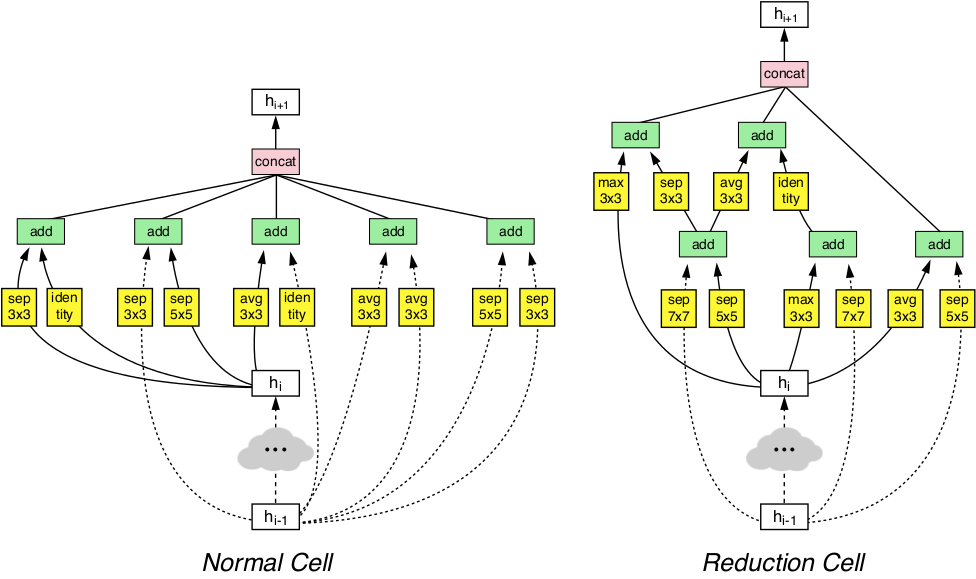
\includegraphics[width=\textwidth]{img/nasnet}
    \caption{Layers used in \textit{NASNet-A}, designed by \textit{AutoML}. Image from \url{ai.googleblog.com/2017/11/automl-for-large-scale-image}.}
    \label{fig:nasnet}
\end{figure}

\subsection{Comparing the classifiers}
At the beginning of this chapter, we mentioned that the classification networks are often compared based on performance on the \textit{ILSVRC} dataset. Newer models like \textit{Xception}, \textit{NASNet}, and modifications of \textit{ResNet} reach excellent accuracy. However, there is a large discrepancy in their performance considering inference speed. In \cref{fig:cnnbenchmark} we provide an overview of fps-accuracy relationship taken from an independent benchmark by Bianco et al. \cite{bib:cnnbenchmark}. Although the experiment was performed with batch size 1, we expect a universal increase of fps with a bigger batch and only small changes to the relative performance of different models. We can observe a clear trade-off between speed and accuracy for the classification task.

\begin{figure}
    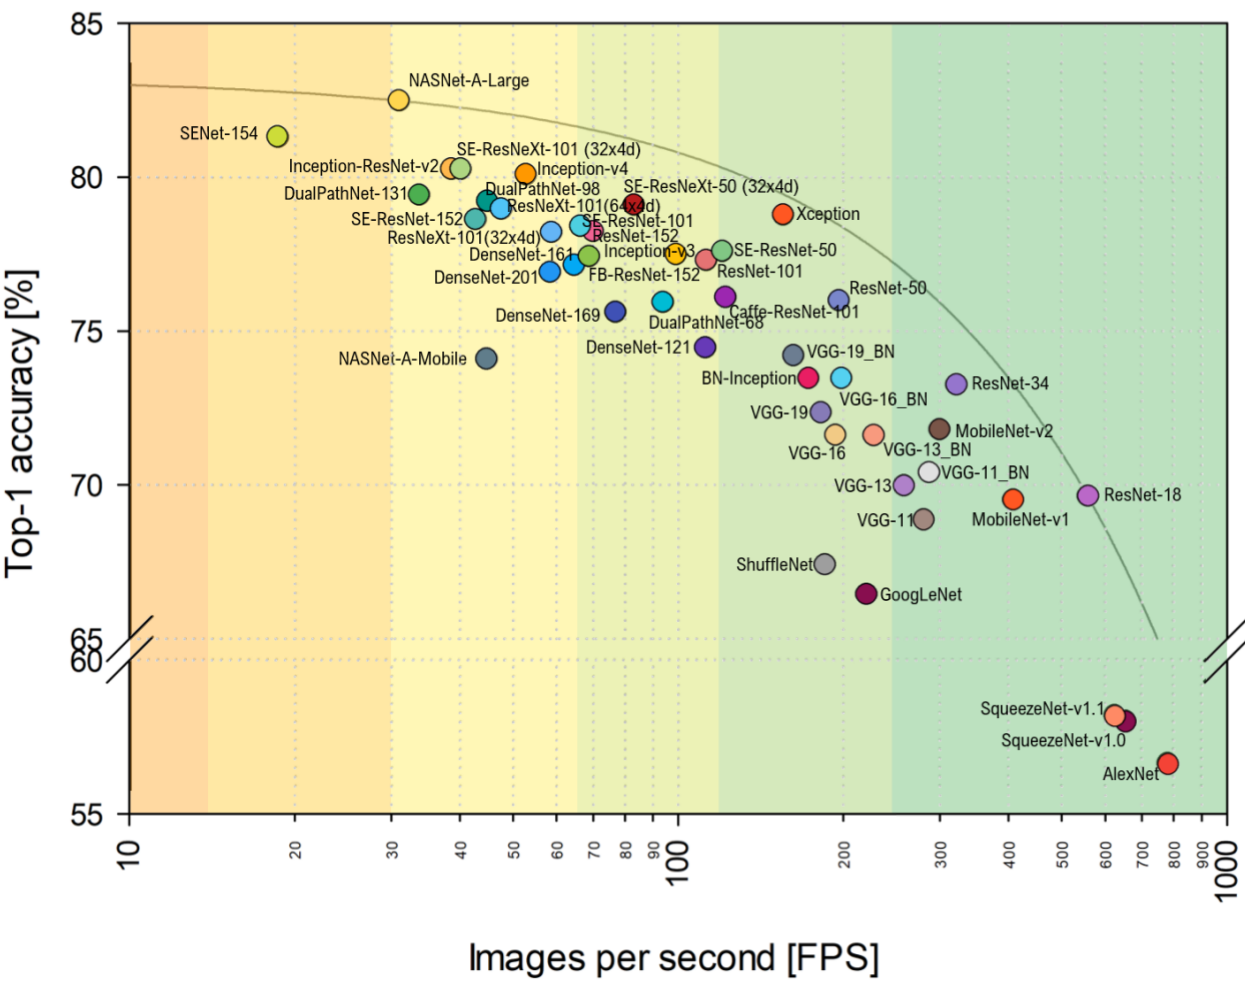
\includegraphics[width=\textwidth]{img/fps_comp}
    \caption{Benchmark of state-of-the-art classification deep neural networks on \textit{ILSVRC} dataset. Performed on NVIDIA
Titan X GPU with batch size 1. Taken from \cite[fig. 3]{bib:cnnbenchmark}}
    \label{fig:cnnbenchmark}
\end{figure}



\section{Detection networks}
\label{sec:detnets}
bla bla bla
\todo{bla}

\subsection{Region-based Convolutional Network (R-CNN) (2014)}
\textit{R-CNN} \cite{bib:rcnn} is the first member of the family of region-based detection models, with iterative improvements in speed and accuracy. The cornerstone idea is simple, select regions in the picture and classify each region. This approach leads to a combination of three modules: region proposal algorithm, feature extraction using CNNs on those regions and classification. 

A naive approach would use a sliding window and classify each cutout of the image.  This approach would be extremely slow, considering different sizes and aspect ratios of possible objects. R-CNN solves this problem by applying a region proposal algorithm and selects about 2000 most likely locations of objects. Regions are selected using the \textit{Selective search} (SS) \cite{bib:selectivesearch} algorithm and serve as a candidates for bounding box predictions.

Each region is then separately processed by a CNN into a feature map. The original architecture uses \textit{Alexnet} CNN, but any classification network can be substituted. Finally, each feature map is scored. Instead of using a soft-max classification provided by classification CNNs, class specific linear support-vector machines are used. Additionally, bounding box regression can be trained to improve prediction accuracy. \Cref{fig:rcnn} illustrates the architecture.

\begin{figure}
    \centering
    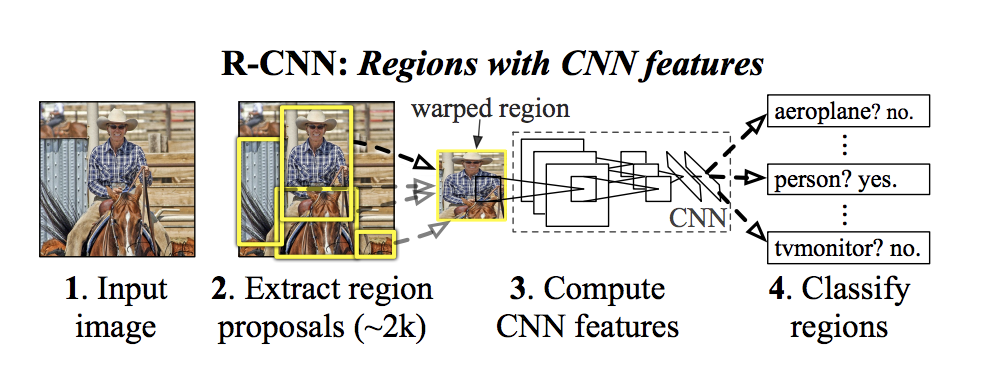
\includegraphics[width=\textwidth]{img/rcnn}
    \caption{R-CNN architecture. Taken from \cite[fig. 1]{bib:rcnn}.}
    \label{fig:rcnn}
\end{figure}

\subsection{Fast R-CNN (2015)}
Even though \textit{R-CNN} was a major step in the right direction, it was still far away from real-time detection. \textit{Fast R-CNN} \cite{bib:fastrcnn} introduces a series of innovations to its predecessor, aimed at improving speed and accuracy. Benchmark on the NVIDIA K40 GPU suggests improvements from 47 seconds per image using \textit{R-CNN} with \textit{VGG-16} feature extractor, to 320 milliseconds with \textit{Fast R-CNN} using the same feature extractor, not including a time for SS proposals. 

Similarly to \textit{R-CNN}, this architecture needs region proposal algorithm, and a CNN to produce a feature map. A drawback of \textit{R-CNN} was computing feature map for each region, despite overlaps. \textit{Fast R-CNN} processes whole input image into a feature map, and then, using a region of interest (RoI) pooling layers, extracts a feature vector for each region. All extracted feature vectors have the same size and are passed through a series of fully connected layers, leading to softmax classifier and bounding box regression layer. An illustration of this process can be seen on \cref{fig:fastrcnn}.

\begin{figure}
    \centering
    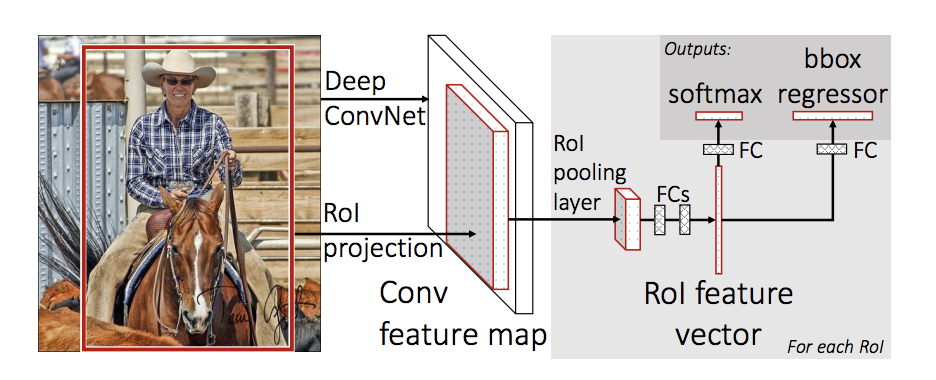
\includegraphics[width=\textwidth]{img/fastrcnn}
    \caption{Fast R-CNN architecture. Taken from \cite[fig. 1]{bib:fastrcnn}}
    \label{fig:fastrcnn}
\end{figure}

\subsection{Faster R-CNN (2015)}
 
 \textit{Faster R-CNN} \cite{bib:fasterrcnn} builds further on the \textit{Fast R-CNN} with the aspiration to achieve a real-time performance. \textit{Fast R-CNN} managed to build a fast feature extraction and subsequent classification usable in a real-time environment but is heavily slowed down by a region proposal SS algorithm. \textit{Faster R-CNN} expands on the idea of sharing resources and replaces SS with \textbf{region proposal network} (RPN). RPN is built on top of a feature map generated by the feature extractor. As suggested, the feature map is shared between RPN and object detection. This approach is able to achieve 5 fps, which can be considered a real-time performance. Whole architecture can be seen on \cref{fig:fasterrcnn}. 
 
 RPN is designed to be a small, sliding-window network, with negligible cost compared to the feature extractor. It is composed of 3$\times$3 convolutional layer with 512 filters and two sibling 1$\times$1 convolutional layers for region regression and classification. Classification in RPNs measures whether proposed region contains a object or a background (\textit{cls} score). Region regression part of the network is tied to the concept of \textbf{anchors}. The anchor is a predefined box centered at a location of sliding-window. \textit{k} such boxes with different sizes and aspect ratios are used. Regression produces 4k parameters relative to anchors, and classifier 2 scores per each anchor. The number of regions is then reduced by eliminating proposals with high overlap using a non-maximum suppression (NMS) based on \textit{cls} score. After NMS, top-N ranked proposal regions are used for detection.
 
 To calculate loss and train RPN, a matching between ground-truth boxes and generated region proposals needs to be determined. A positive label is assigned to two kinds of regions: the ones with the highest IoU overlap with ground-truth box; regions that have IoU higher than 0.7 with any ground-truth box. A negative label is assigned to a non-positive box if its IoU is lower than 0.3 for all ground-truth boxes. Rest of the boxes do not contribute to training. 
 
 The whole model is trained using a 4-step alternating training:
 
 \begin{enumerate}
     \item train RPN initialized with ImageNet pre-trained model
     \item train separate \textit{Fast R-CNN} using proposals generated by RPN from step 1
     \item train RPN with feature extractor initialized by weights learned by the detector in step 2, fine-tune only layers unique to RPN
     \item using the model from step 3, fine-tune layers unique to \textit{Fast R-CNN}
 \end{enumerate}

Thanks to the modular architecture, \textit{R-CNN} networks can exploit any CNN as a feature extractor.  Therefore \textit{Faster R-CNN} can achieve state-of-the-art detection results exploiting the latest advances in classification networks and is often used as a benchmark of their performance.
     

 \begin{figure}
     \centering
     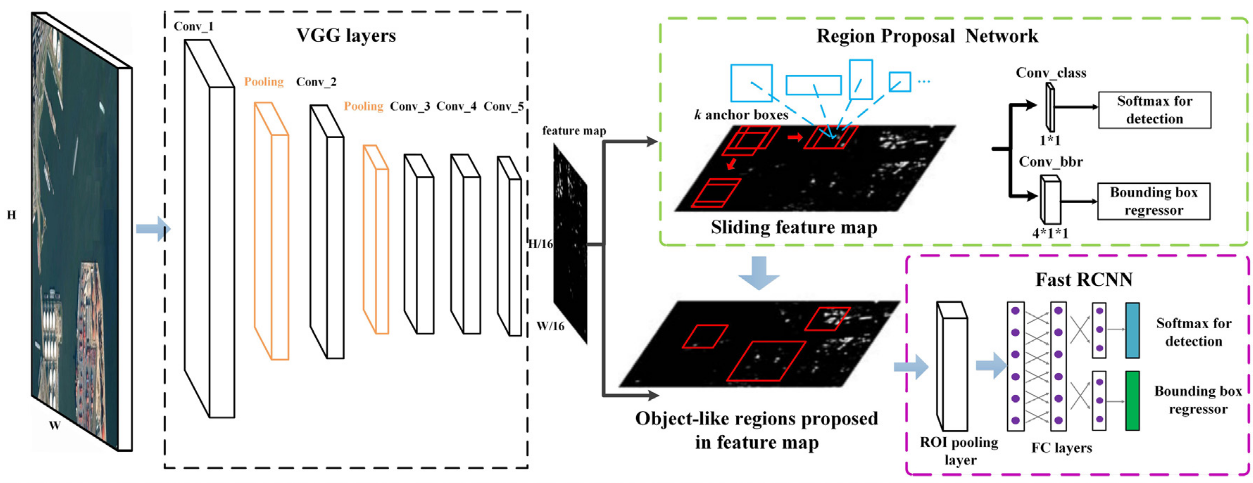
\includegraphics[width=\textwidth]{img/fasterrcnn}
     \caption{The architecture of Faster R-CNN. From \url{https://researchgate.net/figure/The-architecture-of-Faster-R-CNN\_fig2\_324903264}.}
     \label{fig:fasterrcnn}
 \end{figure}

\subsubsection{Mask Region-based Convolutional Network (Mask R-CNN) (2017)}
\cite{bib:maskrcnn}

\subsection*{You Only Look Once (YOLO)}
\subsubsection{YOLO}
\label{sec:yolo}
\subsubsection{YOLO v2 and YOLO 9000}

\subsection*{Single-Shot Detector (SSD)}
\label{sec:ssd}
\subsubsection{SSD}
\subsubsection{FSSD}
\subsubsection{RFB}


%Optional section
% \section{Other uses of CNNs}
% \subsection{Noise removal/ Regularization}
% \subsection{Image generation}


